%---------- Inleiding ---------------------------------------------------------

\section{Inleiding}%
\label{sec:inleiding}

% Rope skipping is een evoluerende jurysport. Jaar na jaar neemt de concurrentie toe met moeilijkere en meer gevarieerde skills. 
% Door de toenemende populariteit van beeldherkenning, krachtigere CPU's en GPU's, en toepassingen die objecten in afbeeldingen herkennen \autocite{Singh_Gill_2022} 
% of acties in video's detecteren \autocite{LUQMAN_2022}, werd zich afgevraagd of dit ook van toepassing kan zijn op meer gecompliceerde en gevarieerd beeldmateriaal.
    
% Op rope skipping competities worden winnaars bekroond door een panel  juryleden die de freestyle van een springer beoordelen. Door groeiende concurrentie, meer gevarieerde trucs, snellere uitvoering en stijgende moeilijkheidsgraad, wordt het jureren lastiger. We onderzoeken of huidige \emph{computer vision}~\ref{subsec:computer vision} technieken klaar zijn om op basis van beeldmateriaal skills te herkennen en deze in te zetten om de objectiviteit en correctheid van scores te verhogen. Verder kan de trucherkenning gebruikt worden om de toeschouwer meer transparantie te bieden de puntentelling, door een replay af te spelen met skill- en scorebenoeming.

Jump rope evolving sport.
Year after year, an increasing amount of high level competitors are pushing the limits of jump rope.
% TODO : source?
Resulting in new skills, new combinations, better phyiques, beter rope material, faster movements.
In order for the judges to keep up with the jumpers and to correctly asses scores to a routine, Double Dutch freestyles are replayed at half speed on International competitions or even locally in Belgium.

Head judges around the world question the best way to correctly judge athletes as to give an accurate ranking on national or international competitions.
Many solutions have been provided: other judging rule-set, splitting judge responsibility, replaying the routine at half speed...
However, with the increasing popularity of image recognition, more powerful computers, applications that recognize objects in images \autocite{Singh_Gill_2022} or applications detecting simple human actions \autocite{LUQMAN_2022}, they wondered about the possibility to incorporate Artificial Intelligence into jump rope to assist judging routinees.
% TODO : Footnote judge ruleset
% TODO : Footnote Double Dutch Freestyle

\subsection{Hoe wordt bepaald hoe skippers presteren t.o.v. elkaar?}

Rope Skipping bestaat echter uit verschillende onderdelen, zoals single rope (SR), chinese wheel (CW) en double dutch (DD). Daarbij zijn er individuele en teamwedstrijden waardoor onderdelen nog verder op te verdelen zijn volgens het aantal springers op het veld, e.g. SR, SR2, SR4, DD3 of DD4. Skippers maken een choreografie van 60 tot 75 seconden en demonstreren dit op de wedstrijd voor het jurypanel. Zij beoordelen de creativiteit (crea) of de moeilijkheidsgraad (difficulty - diff). Een mooie uitvoering, dynamische oefening, springen op muziek, gebruik maken van accenten en trucvariatie behoren allemaal tot het crea-element van de oefening. Voor moeilijkheidsgraad noteren ze per uitgevoerde skill het op basis van het \textbf{juryreglement}, een document dat beschrijft skills een bepaald level krijgen. Aan het eind van de routine worden levels opgeteld, elk level heeft zijn eigen numerieke score die het eindresultaat geven.

\subsection{Wat zijn de uitdagingen bij het jureren vandaag?}

Zoals eerder vermeld verbeteren skippers op fysiek en technisch vlak. Skills variëren meer en worden moeilijker. Voor het onderdeel single rope moet iedere springer dezelfde truc uitvoeren, echter wordt het complexer bij double dutch, daar worden scores toegekend per 'snapshot'. Het jurylid moet draaiers, springers en touwsnelheid tegelijk in het oog houden. Elk van de drie vermelde aspecten levert potentiële levels op en kan elkaar snel opvolgen.

\subsection{Welke technieken kunnen we toepassen om de herkenning van skills te verbeteren?}

Om alles zo goed mogelijk te jureren worden double dutch oefeningen op A-competities herbekeken. Dit is echter limiterend, aangezien er meer juryleden nodig zijn of meer tijd per routine, maar dagen zijn beperkt.
Om dit probleem op te lossen werd aan veel gedacht. Choreografieën op voorhand doorsturen is te veel voorbereiding voor het jurylid. Daarbij duurt het begrijpen van de beschreven skill vaak langer dan het visueel te zien.
Daarnaast zijn eventuele wijzigingen in het jurysysteem weer belastend voor de springer en het jurylid. Immers wordt het geven van levels soms een reflex, dit kan voor foutieve resultaten zorgen bij wijzigingen.
In het nieuws komen soms nieuwe A.I. tools die inspireren. Voorbeelden van beeldherkenning duiken op; zelfrijdende auto's, gebarentaal herkenning, emotiedetectie en de nextJump Speedcounter. Hierdoor de vraag; ``Zijn huidige computer vision technieken voldoende voor het herkennen van rope skipping skills?''

\subsection{Leren uit beeldmateriaal, Proef of concept}
\begin{itemize}
    \item \textbf{Machine learning heeft data nodig. Wat is beschikbaar en hoe kunnen we de accuraatheid van skills meten?}
    De voorkeur voor een oplossing ligt bij het toepassen van machine learning op opnames van recente competities. Daarnaast zijn er tal van beelden te verzamelen van social media. Daarnaast kunnen eigen opnames van voorgaande en toekomstige wedstrijden de accuraatheid van het proefconcept verhogen.
    
    \item \textbf{Wat moet het proefconcept kunnen?}
    Het experiment moet de verschillende skills in een gegeven video benoemen en eventueel aangeven hoe zelfzeker het is. Hiervoor hebben alle trucs een eenduidige classificatie nodig die alle unieke combinaties van elkaar kunnen onderscheiden.
\end{itemize}

\subsection{Onbeantwoorde vragen}

Naast de inleidende deelvragen zijn er nog onbeantwoorde vragen. Hiervan vind je hieronder een oplijsting en worden verwerkt als antwoord in de resultaten of conclusie. Om daartoe te bekomen vind je in wat volgt een literatuurstudie naar de recente technieken die we kunnen gebruiken voor het herkennen van skills en de uitdagingen ervan. Nadien volgt het plan van aanpak, de verwachte resultaten en tot slot de conclusie, maar eerst de deelvragen.

\begin{itemize}
    \item Wat is het beste model om de trucs te herkennen?
    \item Hoe wordt het model opgebouwd?
    \item Wanneer zijn voorspellingen goed genoeg om te dienen als extra jurylid of als steunmiddel?
    \item Kunnen we de AI-Judge gebruiken om juryleden te verbeteren?
    \item Indien het proefconcept een oefening kan jureren, kunnen we hieruit afleiden dat dit voor alle jurysporten kan? Indien wel, wat zou de beste aanpak zijn?
\end{itemize}

%---------- Stand van zaken ---------------------------------------------------

\section{Literatuurstudie}%
\label{sec:literatuurstudie}

% TODO: (TAAL controle literatuur)

% TODO BP: volgorde en uitbreiding literatuur.
% Convolutielagen in een nutshell -> van matrix naar matrix (afbeelding), maar cellen van een nieuwe matrix zijn een som van andere rijen en kolommen (initieel pixels)
% LSTM in een nutshell -> geheugencellen, activatiefunctie -> input, memory, activativering output.
    
Het onderzoek naar skillherkenning wordt stapsgewijs opgebouwd. Beginnen doen we met een introductie en definitie van skills, waarna gepast onderzoek naar technieken kan gebeuren. Stilaan bouwen we dit op tot we beter definiëren waar de moeilijkheden liggen bij het herkennen van skills om zo de gevonden modellen te verfijnen tot het gewenste resultaat.

\subsection{Skills intro}
\label{subsec:basisskills}

    Eerder beschreven we al de aanwezigheid van verschillende onderdelen in Rope Skipping. Om het onderzoek doenbaar te houden, leggen we de focus op single rope individuele freestyle (SR) en double dutch single freestyle (DD3). Beide onderdelen hebben een ander jurysysteem, waarbij verschillende elementen terugkeren, maar ook anders zijn. Soms wordt ook enkel over SR gesproken om niet in herhaling te vallen.

\subsubsection{Single Rope}

Bij single rope spring je alleen in het touw. De trucs die je kan uitvoeren zijn te verdelen in verschillende categorieën: gyms G, powers P, wraps W, releases R, backwards B, multiples M, crosses C, footwork F, Interactions I (in het geval van SR2) en een quasi eindeloze combinatiemogelijkheid. Waarbij multiples al een combinatie zijn van crosses, maar dan meerdere touwrotaties in één sprong. Ook kan je een wrap met een release combineren, multiples landen in powers, release kan uitvoeren in een multiple en dit nog eens allemaal achteruit.
Enkele voorbeelden:

% TODO : bijlage bij BP
\begin{itemize}
    \item Crosses
    \begin{itemize}
        \item side swing (s - zwaai naast het lichaam)
        \item open (o - gewone sprong)
        \item kruis (c - standaard kruising op de buik)
        \item toad (knie heffen, één arm onder je been)
        \item EB (arm buik + arm op rug)
        \item AS (armen gekruist achter de knieën)
        \item CL (één arm achter de knieën, de andere op de rug)
        \item TS (beide armen op de rug)
    \end{itemize}
    \item Multiples
    \begin{itemize}
        \item dubbel - DU - 2 rotaties
        \item triple - TU - 3 rotaties
        \item quad - QU - 4 rotaties
        \item quint - 5 rotaties
        \item TU.sEBo - eerst rotatie side, dan EB en tot slot openen
    \end{itemize}
    \item Powers
    \begin{itemize}
        \item push-up - naar plankhouding gaan en bij het rechtkomen het touw onder de voeten trekken.
        \item split - idem push-up
        \item frog - handstand
    \end{itemize}
\end{itemize}

Op die manier kunnen categorieën gecombineerd worden. We kunnen zelfs verder gaan. Zo kan je een TU.sEBo landen in push-up enzovoort.

\subsubsection{Double Dutch}
Bij dubbel dutch zijn er steeds twee draaiers en minstens één springer. De elementen zijn gelijkaardig, maar toch een beetje anders. Voor de categorieën blijven Gymnastics, Powers en Footwork over. Bijkomend heb je overgangen (Switches) en draaierstrucs (Turners). Zo kunnen draaiers normaal of in restrictie draaien. (toad, kruis, EB, TS\dots)
Voor het geven van levels wordt er gekeken naar 'snapshots' of momentopnames. Het level wordt dan skill(overgang) van de springer + het level van de draaiers + het level voor rotatiesnelheid (dubbel, tripel\dots).
    
Zoals in elk onderdeel kunnen fouten gebeuren, dit is een stop van het touw, die een negatieve beïnvloeding hebben op de score.

\subsection{Computer vision}
\label{subsec:computer vision}

Om de skills automatisch te herkennen hebben we input nodig, data. Online zijn er reeds vele video's te vinden, maar ook eigen opnames en die van Gymfed/Arne zijn beschikbaar, waardoor de keuze om te leren uit beelden snel gemaakt werd. Het studiegebied waarbij computers kenmerken, personen of andere objecten in digitaal beeldmateriaal herkennen, noemt men computer vision. Meer specifiek ligt de focust bij het herkennen van menselijke activiteiten in deze beelden, ook wel human activitity recognition of HAR \autocite{Pareek_2020}.
Voor het herkennen van mensenlijke activiteiten worden ook Human Gait Recognition, HGR, of Human Pose Recognition, HPR, gebruikt. Hoewel de drie technieken dicht bij elkaar aanleunen, hebben ze elk een andere nuance. HGR kijkt naar de typische bewegingen, gestiek of gedragspatronen van een mens \autocite{Alharthi_2019}, terwijl HPR specifieke kijkt naar poses of speciale uitdrukkingen \autocite{Song_2021}. Ze vertellen ook hoe poseherkenning, skeletgebaseerd, als hulpmiddel kan gebruikt worden zijn om het labelen van activiteiten te verbeteren.


\subsection{Uitdagingen}
\label{subsec:uitdagingen}

Naast de drie gebieden van menselijke herkenning, gestiek, acties en poses, beschrijven \textcite{Pareek_2020} een andere verdeling; gestiek, acties, interacties en groepsactiviteiten. De laatste twee vergen nader onderzoek bij het verhogen van de accuraatheid van teamoefeningen. Verder vertellen ze de uitdagingen van dimensionaliteit, grootte van de videobestanden, similariteit van de acties etc en voorzien ze een algemeen overzicht voor human activity recognition. \textcite{Issa_2023} beschreven hoe ze een video tot één vector reduceerden met kenmerken om een LSTM-model te vermijden, een model dat aan de hand van geheugencellen gespecialiseerd is in het verwerken van sequentiële data. Hoewel de accuraatheid van 68 tot 74\% minder is dan volgend beschreven methoden, kan dit een handig inzicht zijn voor later.


\subsection{Herkennen van de atleet}
\label{subsec:herkennen van de atleet}

Het eerste doel van het proefconcept is het herkennen van de springer. \autocite{Zaidi_2021} deed een onderzoek naar de moderne deep learning technieken voor het herkennen van objecten en besprak verscheidene modellen, zoals YOLO, SSD, CenterNet, CNN, hun varianten en de nood aan compactere modellen voor dagelijks gebuik. Echter vergt het onderzoek niet het herkennnen van rope skippers op één afbeelding, maar gedurende de gehele video of videofragmenten. Om dit proces mogelijk te vereenvoudigen vergelijkt \textcite{Gao_2022} recente deep learning technieken die de voor- en achtergrond in video's van elkaar onderscheiden, genaamd video object segmentation of VOS. Gaande van het herkennen van een persoon, tot het herkennen van armen, benen, voeten, handvaten en touwen. Hoewel \textcite{Bharadiya_2023} aangeeft dat CNN kenmerken herkent ongeacht de positie in de afbeelding, zouden we de gemaskeerde beelden kunnen schalen en centreren. Vooral bij wedstrijddata springen atleten dichtbij of ver in het veld ten opzichte van de camera. In het volgende deel kunnen we dit dan gebruiken voor volledige trucherkenning.
    

\subsection{Skillherkenning}
\label{subsec:skillherkenning}

Voor herkennen van acties verschenen de laatste jaren verschillende combinaties die het Long Short Term Memory neuraal netwerk (LSTM) combineren met het convolutional neural network (CNN). \textcite{LUQMAN_2022} maakten zo een CNN-LSTM waarbij de video's eerst door convolutielagen gingen en nadien pas door de LSTM lagen. Ook \textcite{Sun_2023} en \textcite{Ullah_2024} gebruikten deze structuur voor het herkennen van voorgekookte pastatypes of classificatie van een tennisacties, respectievelijk a.d.h.v. infrarood of beeldmateriaal.
Omgekeerd bereikten \textcite{Xia_2020} met hun LSTM-CNN architectuur scores van 92-95\% op drie populaire publieke datasets UCI, WISDM en OPPORTUNITY en in \textcite{Aksan_2023} werden het LSTM, CNN, CNN-LSTM en LSTM-CNN met elkaar vergeleken op hoogspanningsnetdata als case study. Daarentegen vergeleken \textcite{Ellouze_2024} de geconcateneerde versie met een hybride versie, genaamd het convolutional LSTM, waarbij de convolutionele operator verwerkt zit in het LSTM netwerk zelf, met betere prestaties tot gevolg. Ook in \autocite{Sharma_2023} werd dit toegepast met behulp van een skeletextractie (HPR), waarbij de lichaamskenmerken, armen, ellebogen, knieën etc. in kaart werden gebracht als skelet en als parameter in het model werd toegevoegd. Nochtans kwamen \textcite{Lin_2020} in 2020 al met een Self-Attention ConvLSTM (SAM) die betere resultaten gaven dan andere convolutional LSTM samenstelling en vergeleken ze hun model met \textcite{Wang_2019}'s Memory in Memory model.

\subsection{SAM \& MIM}
\label{subsec:SAM&MIM}

\textcite{Wang_2019} onderzochten een verbetering voor de huidige modellen voor tijdruimtelijke data. Ze vonden dat LSTM-geheugencellen te simpel waren om complexheden van hogere orde te bevatten. Hierdoor ontwierpen ze een memory in memory component, ter vervanging van de normale geheugencel, die datasets met een hogere moeilijkheidsgraad beter konden voorspellen. Hieruit vloeide de naam Memory in Memory, MIM.
\textcite{Lin_2020} daarentegen gebruiken een self-attention memory cell binnenin het convLSTM die globale aspecten in de tijd en ruimte kan onthouden. Met ongeveer 35\% het aantal parameters t.o.v. Wang's MIM, bereikte SAM een gelijkaardige score als op o.a. de movingMNIST dataset, maar sneller. Hoewel de focus van deze papers lagen op het voorspellen van toekomstige acties, kan de output weer omgevormd worden, naar een classificatie i.p.v. een voorspelling.


\subsection{Skill complexiteit \& levels}
\label{subsec:skillcomplexiteit}

Eerder werd al een basisuitleg van skills gegeven, met enkele voorbeelden. Om alle skills te herkennen dienen ze zo goed mogelijk uitgewerkt te worden. Dit deel legt de basis uit van het levelsysteem volgens de Gymfed juryreglement 2023-2024.
Een kruis, toad, of crouger zijn 'voorwaartse' skills die uitgevoerd worden zonder een voorbereidende rotatie, er zijn geen restricties achter het lichaam waarbij een voorbereidende rotatie nodig is. Trucs waarvoor dit wel geldt zijn bijvoorbeeld AS, CL, TS of meghan, ze bestaan uit het gaan naar en komen uit, om de volledige skill uit te voeren. Scores worden gegeven aan de hand van levels, zo krijg je per restrictie van de armen een level. Zo krijg je voor een toad, crouger en EB 1 level, terwijl een TS, elephant of CL 2 levels oplevert.
Gewone kruisjes zijn te eenvoudig en leveren niets of slechts een half level op en zijn verder niet additief bij combinaties. Combineer je veelvuldig zo basisoefeningen tot een reeks, dan krijg je voor iedere unieke overgang het level. Bijvoorbeeld;

\begin{itemize}
    \item toad-crouger-toad (1-1-1)
    \item toad-toad-toad (1-1-herhaling)
    \item CL en even later toad-CL (1-2) mag ook, ook al kan je niet rechtstreeks van toad naar CL
\end{itemize}

Wissel je bovendien van armen, switch crosses, aangeduid met een x, dan krijg je 1 of 2 extra levels.

\begin{itemize}
    \item toad-xtoad (1-2)
    \item AS-xAS (2-4)
    \item AS-CL (2-2)
    \item AS-xCL (2-3)
\end{itemize}

Al deze crosses kan je combineren met andere categorieën. Met 2 springers kan je iemand meenemen in een toad, kruis of TS, multiples worden opgebouwd uit unieke rotatiecombinaties. Voor quads komt dit bijvoorbeeld neer op:
\begin{itemize}
    \item QU.s.o.AS.o (QU = 3, AS = 2, totaal = 5)
    \item QU.s.AS.o.o (5)
    \item QU.s.c.AS.o (5)
    \item QU.s.EB.AS.o (6)
\end{itemize}

Bovendien kunnen deze skills gecombineerd worden met powers, releases of achteruit gesprongen worden en zijn er nog een aantal speciale gevallen of uitzonderingen die minder of extra punten opleveren. Dit brengt ons to het volgende onderdeel video segmentation en branching.

\subsection{Skillafbakening \& branching}
\label{subsec:video segmentation & branching}

In \textcite{Zahan_2023} wordt het standaard LSTM uitgebreid om beter langdurige informatie te verwerken om resultaten van gehele gymnastiekoefening te voorspellen. Aangezien het jurysysteem van die data hierdoor één-op-één gekoppeld is aan het model, is dit niet robuust genoeg voor veranderende versies. Het proefconcept wenst dus de skills te leren waarop de levels gemapt worden via een functie.
    
Om alle trucs en combinaties van elkaar te onderscheiden werd stap per stap een skillmatrix opgebouwd. Deze matrix tracht zo veel mogelijk, om niet te zeggen alle, oefeningen op te delen volgens kenmerkende eigenschappen. Dit denkproces bracht de afbakening van skills en combinaties in kaart.
Freestyles en ander beeldmateriaal moet gesplitst worden in eenduidig, atomair benoembare (sub-)skills, minivideo's, die slechts één representatieve voorstelling hebben in de skillmatrix.
Concreet betekent dit dat na afbakening van skills, iedere mini-video, nog herstelbaar moet zijn tot zijn combinatie.
Doorgaans geeft het verlaten van de grond aan dat een truc begint, analoog bij het landen en in de lucht zijn. Dit is echter niet altijd het geval bij wraps of releases. Tevens moeten de geknipte video's, na de afbakening van de trucs, even lang zijn (gelijke dimensies). Een simpele truc hiervoor is het toevoegen van \emph{lege} informatie, zwarte frames, genaamd padden (Engelse term). Vaak zullen langdurige intervallen wraps of herstel van fouten zijn. Deze lange sequenties kunnen apart gemodelleerd worden of verder opgesplitst om de padding niet te lang te maken.

\subsubsection{Skillmatrix}

De de skillmatrix is voor verandering vatbaar, wanneer combinaties ontdekt worden die er niet in passen en ziet er op dit moment voor single rope als volgt uit:

\begin{itemize}
    \item \textbf{Beschrijving}: louter informatief
    \item \textbf{Puntnotatie}: eigen notatie voor bestandsbenoemingen, nog niet optimaal met wraps, ongeveer skillmatrix in compacte vorm
    \item \textbf{Categorie}: I, G, P, W, R, B, M, C, F
    \item \textbf{Personen}: aantal skippers die de skill hebben uitgevoerd, soms 3 van de 4 bij een teamoefening
    \item \textbf{Rotaties}: aantal rotaties van het touw, 0-7, 0 bij gaan naar of valse powers of wrapjes
    \item \textbf{Touwrichting eerste rotatie}: voorwaarts, achterwaarts, zijwaarts eventueel voor buddybounce
    \item \textbf{Touwrichting laatste rotatie}: idem
    \item \textbf{touw rot wissels}: 0 of 1, theoretisch 2, 3, 4 mogelijk
    \item \textbf{PLR}: 0,1,2+ parallelle lichaamsrotaties met grond (e.g. crab rond body as, evt. frog to crab niet doorsteken, pushup body-as)
    \item \textbf{LLR}: 0.25 -> 2+ loodrechte lichaamsrotaties met grond (e.g. hummingbird, 360, halve draai, turn table crab, turn table pushup)
    \item \textbf{multiplepart} 8x gedupliceerd, invulling per rotatie van de multiple, wrapstatus, powers landen in multiple \dots
    \begin{itemize}
        \item \textbf{categorisch} s, o, c, toad, EB, AS, TS, knie, open-toe, mic, 1-H-release, powers, gyms \dots
        \item gaan naar (AS, wrap op), komen uit (AS, unwrap), switch cross (ASxAS), sticky (AS-AS)
        \item \textbf{wrapped bodyparts}: arm, been, tussen been rond arm...
        \item \textbf{Interaction type}: schep, pak voor, pak achter
        \item \textbf{combinatietype}:
        \begin{itemize}
            \item pre skill: multiple landen in power
            \item mid skill: e.g. salto met multiple of release, release while wrapped
            \item post skill: e.g. power doortrekken in kruis of multiple
        \end{itemize}
    \end{itemize}
\end{itemize}

    
Meteen valt te zien dat er theoretisch veel meer mogelijkheden zijn dan die daadwerkelijk gesprongen. Wraps kunnen eventueel nog buiten beschouwing gelaten worden aangezien deze niet moeilijk te jureren zijn, maar moeilijker eenduidig te benoemen.

Verder zie je een soort hiërarchische structuur opduiken. We kunnen hiermee twee kanten opgaan. Ofwel beschouwen we het geheel als alle mogelijke klassen die we kunnen voorspellen en wensen we meerdere labels te geven in zijn geheel, ongeveer 1 label per categorie, rotaties, PLR, combinatietype\dots als een , ofwel passen we een soort branching toe per onderdeel zoals \textcite{Coulibaly_2022} beschreven in sectie 4.4.1. Immers draaien we ofwel voorwaarts, ofwel achterwaarts.
Dit kan potentieel de accuraatheid bij meerdere springers verhogen, één branch per atleet.

\subsection{Samenvatting literatuurstudie}
\label{subsec:samenvatting literatuur}

Het proefconcept moet rope skipping skills labelen uit videos. Vele video's, namelijk freestyles, bestaan uit verschillende skills die elk een level krijgen, voorbehouden aan wijzigingen in het juryregelement. De freestyles dienen geknipt te worden in minivideo's per skill die op hun beurt weer een label toegekend krijgen aan de hand van de skillmatrix waarbij meerdere springers mogelijk zijn in het geval van DD3.


% Refereren naar de literatuur kan met:
% \autocite{BIBTEXKEY} => (Auteur, jaartal): voor een referentie tussen
% haakjes, waar de auteursnaam GEEN onderdeel is van een zin.
% \textcite{BIBTEXKEY} => Auteur (jaartal): voor een narratieve referentie,
% waar de naam van de auteur effectief een onderdeel is van de zin.


%---------- Methodologie ------------------------------------------------------
\section{Methodologie}%
\label{sec:methodologie}

Aan dit proefconcept kan rustig gewerkt worden in de zomer en veel in het tweede semester, (geen stage, enkel BP, ITP\&CO, Data science en big data). Aangezien het labelen veel tijd in beslag kan nemen, zal dit iteratief en semi-supervised gebeuren doorheen het onderzoek, gefocust op individuele skills (SR) en double dutch single freestyles (DD3). Hierdoor zal slechts een deel van de reeds verzamelde 500GB aan beeldmateriaal gebruikt worden. Echter is dit niet het enige beschikbare materiaal. Een ruwe schatting denkt dit aantal nog makkelijk te verdubbelen in de toekomst door online te zoeken en rond te vragen binnen de rope skipping community.
    
Verder wordt het project iteratief opgebouwd. Een eerste diepere duik in de wereld van deep learning werd reeds gemaakt, zoals gezien in de literatuurstudie. Deze zal regelmatig opknapbeurten of aanvullingen krijgen door opduikende moeilijkheden en/of problemen.

\subsection{Iteratief proces}
Om de proef te starten wordt de nieuwe kennis toegepast op een beperkte set video's om deze te bakenen in mini-video's. Nadien wordt de borstel door de huidige data gehaald om er later beter op te kunnen filteren. Zo kunnen we ook statistieken maken die een kleine vergelijking geeft tussen wedstrijddata vs andere data, meest gesprongen truc, club, land, jaar met meeste data\dots
Als volgende moeten de modellen meer performantie bieden, dit kunnen we doen door de dimensionaliteit te verkleinen via en de best mogelijke techniek(en) voor videoherkenning en beter rekening houden met meerdere springers al dan niet door gebruik van één of meerdere VOS technieken. Hierdoor kunnen we de skillafbakening verbeteren en omtoveren tot een semi-supervised model dat stilaan zelf extra trainingslabels voorziet, met verificatie en aanvullingen van trucs.
    
Losse stukken code en probeersels maken de code snel onoverzichtelijk, foutgevoelig en niet bevorderend om te analyseren. Daarom wordt een speciaal moment voorzien die de cohesie, portabiliteit en structuur van de code verbetert. Hieruit volgt dat nadien de volledige focus gelegd kan worden op implementatie van een eerste HAR-model, verfijning en vergelijking met andere modellen om het beste eruit te halen. Tot slot wordt het onderzoek aangevuld met alle de bevindingen, resultaten en de conclusie.
    
In figuur~\ref{fig:../graphics/gantt} wordt een schatting van de tijdsplanning gegeven en in de oplijsting hieronder vind je meer details per fase.

\begin{figure}
    \centering
    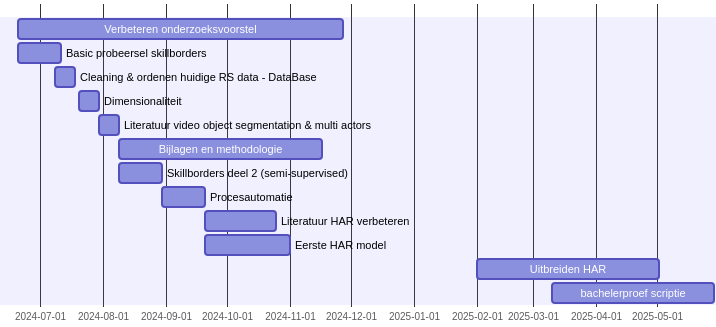
\includegraphics[width=.8\columnwidth]{img/gantt}
    \caption{\label{fig:gantt}Indicatie tijd en indeling per fase}
\end{figure}

\subsection{Fasering}

\begin{itemize}
    \item \textbf{Fase 0: Verbeteren onderzoeksvoorstel}
    \begin{itemize}
        \item \textbf{Doelstelling}: Kwaliteit verhogen
        \begin{itemize}
            \item Structuur begint aan te voelen als: een novel aanpak voor HAR in jurysporten
            \item of
            \item Toepassing van recente HAR technieken op complexere rope skipping data
        \end{itemize}
        \item \textbf{Aanpak}:
        \begin{itemize}
            \item Meer vorm geven aan try-outs en effectieve uitvoering
            \item Extra literatuurstudie, op basis van extra ondervindingen
            \item Blijven bouwen aan dat proefconcept
        \end{itemize}
        \item \textbf{Must have}: Verhoogde kwaliteit (literatuur, proeven)
        \item \textbf{Should have}:
        \begin{itemize}
            \item semi-supervised border labeling
            \item meer kennis over self-attention, lstm memory cells
        \end{itemize}
        \item \textbf{Could have}:
        \begin{itemize}
            \item Een eerste HAR model
            \item afgewerkte HAR- \& dimensionaliteit-literatuur
        \end{itemize}
        \item \textbf{Will not have}: Nieuwe eigen modellen
    \end{itemize}
    \item \textbf{Fase 1: Basic probeersel skillgrenzen}
    \begin{itemize}
        \item \textbf{Doelstelling}: Mini model, standaard CNN en/of LSTM, die door een tiental video's kan proberen om frames aan te duiden die de grens van een skill zijn.
        \item \textbf{Aanpak}:
        \begin{itemize}
            \item Eigen testvideo's verder labelen
            \item Data preprocessing - opsplitsen video's
            \item Train \& test
            \item Bouwen/zoeken visual die de video-opdeling van een nieuwe testvideo kan tonen
        \end{itemize}
        \item \textbf{Resultaat, deliverable(s)}:
        \begin{itemize}
            \item \textbf{Must have}: skillsafbakening in video als oplijsting van framenummers
            \item \textbf{Should have}: Verhoogd begrip computer vision \& skillafbakening
            \item \textbf{Could have}: modelkeuze (LSTM, CNN, YOLO...)
            \item \textbf{Will not have}: Opgeslagen mini-video's
        \end{itemize}
    \end{itemize}
    \item \textbf{Fase 2: Cleaning \& ordenen huidige RS data - database}
    \begin{itemize}
        \item \textbf{Doelstelling}: Opkuisen structuur en huidige video's
        \item \textbf{Aanpak}:
        \begin{itemize}
            \item Aanmaken databank waarbij elke video 'extra' info krijgt, wie, wat, waar, kwaliteit, obstructielevel/ruis, competitie/voorbeeldoefening, landscape/portret, bestandslocatie... (om dubbels te vermijden)
            \item Data van Arne (groot bk, bk 23 en bk 24) herbenoemen
            \item Eigen opnames verder knippen en benoemen
            \item Gescrapete video's herbenoemen
            \item DB voorbereiding skilltabel (mogelijke skills, makkelijk te vinden in video)
            \item DB voorbereiding skillborders voor bevestigde of semi-supervised splits + skill\_key
        \end{itemize}
        \item \textbf{Must have}: alles
    \end{itemize}
    \item \textbf{Fase 3: Dimensionaliteit}
    \begin{itemize}
        \item \textbf{Doelstelling}: Aanvullen literatuurstudie m.b.t. dimensionalieitreductie voor computer vision video machine learning
        \item \textbf{Aanpak}:
        \begin{itemize}
            \item Zoektocht voor specifiek HAR
            \item Lijst van technieken of het best mogelijke
            \item Voorbeeld met convLSTM, SAM of MIM?
        \end{itemize}
        \item \textbf{Must Have}: Minstens één techniek
        \item \textbf{Could have}: Voorbeeld met HAR
        \item \textbf{Will not have}: gecompresseerde video's
    \end{itemize}
    \item \textbf{Fase 4: Literatuur video object segmentation \& multi actors}
    \begin{itemize}
        \item \textbf{Doelstelling}:
        \begin{itemize}
            \item Literatuur multi actors verbeteren
            \item Literatuur VOS longlist technieken
            \item Invloed multi actors op VOS weten
            \item Shortlist van VOS technieken die omkunnen met meerdere actoren
        \end{itemize}
        \item \textbf{Aanpak}:
        \begin{itemize}
            \item Huidige source, multi actoren daarvoor beter doornemen
            \item VOS Technieken zoeken die hiermee om kunnen
            \item Armen, benen, touw, handvaten of enkel het geheel?
            \item Shortlist van maken
        \end{itemize}
        \item \textbf{Must have}: Shortlist VOS
        \item \textbf{Should have}: Techniek die het touw accuraat in beeld brengt
        \item \textbf{Will not have}: 'aparte' video's die door per actor door het HAR-model moet
    \end{itemize}
    \item \textbf{Fase 5: Bijlagen en methodologie}
    \begin{itemize}
        \item \textbf{Doelstelling}: Bijhouden methodologie en bijlagen opstellen
        \item \textbf{Aanpak}:
        \begin{itemize}
            \item Volgen van deze methodologie
            \item Afwijkingen noteren
            \item Bijlagen toevoegen, skillist, skillmatrix met foto's
        \end{itemize}
    \end{itemize}
    \item \textbf{Fase 6: Skillborders deel 2 (semi-supervised)}
    \begin{itemize}
        \item \textbf{Doelstelling}: Verbeteren en vereenvoudigen eigen werk
        \item \textbf{Aanpak}:
        \begin{itemize}
            \item Overschakelen op semi-supervised
            \item Verbeteren probeersel skillgrenzen, m.b.v. VOS \& dimensionaliteitsreductie
            \item Toevoegen grenzen testvideo's - manual, verified, semi-supervised
            \item Zo zorgen testen tussendoor voor extra labels
            \item Toevoegen andere modellen YOLO, SSD...
        \end{itemize}
        \item \textbf{Must have}:
        \begin{itemize}
            \item split video optie
            \item verifieer grenzen (alle, volgens bepaald zekerheidspercentage)
        \end{itemize}
        \item \textbf{Should have}: /
        \item \textbf{Could have}: Verifieer niet bevestigde labels en toon grootste onzekerheden
        \item \textbf{Will not have}: Niet alles moet gelabeld zijn
    \end{itemize}
    \item \textbf{Fase 7: Procesautomatisatie}
    \begin{itemize}
        \item \textbf{Doelstelling}: Verhogen weergave, keuzeopties modellen, begrip en staat van het proefconcept
        \item \textbf{Aanpak}:
        \begin{itemize}
            \item Configuratiebestanden: run info, modelselection, keuze labels train...
            \item Portabiliteit: Docker?
            \item Logs, run en modelstatistieken, datastatistieken
            \item Documentatie
            \item Toevoegen nieuwe video, geeft skillgrenzen en verifieeropties
        \end{itemize}
        \item \textbf{Must have}: portabiliteit, configuratie
        \item \textbf{Should have}: toon meest onzekere niet-geverifieerde skills
        \item \textbf{Could have}: statistieken
    \end{itemize}
    \item \textbf{Fase 8: Literatuur HAR deel 2 (september/oktober)}
    \begin{itemize}
        \item \textbf{Doelstelling}: Extra zoektocht naar HAR-modellen, op het einde van de zoektocht kwam (Lin, 2020) tevoorschijn, beste paper voor HAR tot nu gevonden, maar dat wil zeggen dat er nog 4 jaar aan evolutie kan zijn
        \item \textbf{Aanpak}: zoeken
        \item \textbf{Should have}:
        \begin{itemize}
            \item Extra modellen
            \item Aangepaste shortlist
            \item recenter model
            \item generiek idee hoeveel literatuurstudie er nog bijkomt
        \end{itemize}
    \end{itemize}
    \item \textbf{Fase 9: Eerste HAR model (target september)}
    \begin{itemize}
        \item \textbf{Doelstelling}: Eerste implementatie HAR-model
        \item \textbf{Aanpak}:
        \begin{itemize}
            \item Implementatie van de code van het gekozen model
            \item Volledig begrip van het gekozen model. (Niet blackboxen)
            \item Preprocessing video's, splitsen, VOS, padding
            \item branching vs binaire classificatie voor alle kolommen
        \end{itemize}
        \item \textbf{Must have}: trucvoorspelling
        \item \textbf{Should have}: Keuze optie branch of binair
        \item \textbf{Could have}: Procentuele modelstatistieken (per testrun)
    \end{itemize}
    \item \textbf{Fase 10: Uitbreiden HAR}
    \begin{itemize}
        \item \textbf{Doelstelling}: Verbeteren model \& vergelijkingen
        \item \textbf{Aanpak}:
        \begin{itemize}
            \item Andere v/d twee als optie in config toevoegen: branching of niet
            \item Toevoeging gewenste config opties discovered along the way
            \item Toevoegen modellen SAM, MIM, convST-LSTM
            \item Semi-supervised skills aan trainingsset DB (verified or not)
        \end{itemize}
    \end{itemize}
    \item \textbf{Fase 11: bachelorproef scriptie}
    \begin{itemize}
        \item \textbf{Doelstelling}: Afwerking bachelorproef
        \item \textbf{Aanpak}:
        \begin{itemize}
            \item Bijwerken methodologie
            \item Methodologie finetunen (tussendoor bijhouden)
            \item Conclusie
            \item Dankwoord
            \item Bijlagen finetunen
            \item Inleiding en abstract finetunen, die overeenkomen met literatuur en resultaat
        \end{itemize}
        \item \textbf{Must have}: Alles
    \end{itemize}
\end{itemize}


\subsection{Aanpak beantwoording deelvragen}
\label{subsec:methodologie-deelvragen}

% TODO : finetune this : taal

Om antwoord te geven op de vragen; ``Wanneer zijn voorspellingen goed genoeg om te dienen als extra jurylid of als steunmiddel?'' en ``Kunnen we de AI-Judge gebruiken om juryleden te verbeteren of omgekeerd?'', moet er even samengezeten worden met juryexperten.
Een eigen voorstel is; Na indiening van de score, krijgt het jurylid de levels van een werkend model, die controleert en duidt die levels aan die niet overeenstemmen met de eigen gegeven levels, juryleden kunnen zichzelf ofwel verbeteren, ofwel het model verbeteren. Later kan een overgang gemaakt worden naar meest onzeker skills van het model verifiëren.

De deelvraag over de veralgemening tot jurysporten zal moeten afwachten op het verloop van het proefconcept.

\subsection{Training \& Hardware}

Werken met beeldmateriaal alleen al vraagt veel resources, laat staan het trainen op de data met een normale laptop. Best wordt er gewerkt met één of meerdere GPU's om het onderzoeksproces te bevorderen. Tussendoor kunnen berekeningen gemaakt worden om in te schatten hoe lang trainsessies zullen duren. Tevens geeft dit ook toekomstige referentie voor andere computer vision concepten.


%---------- Verwachte resultaten ----------------------------------------------
\section{Verwachte resultaten}
\label{sec:verwachte-resultaten}

    Het PoC is veel werk, in het goede geval wordt alles perfect afgewerkt. Het is uitbreidbaar en in te krimpen. Zo kan SR of DD3 overgeslagen worden tot slechts één onderdeel of kan de skillafbakening meteen zorgen voor problemen. Echter bleek uit de literatuurstudie dat dit wel moet lukken. Ook voor het herkennen van trucs zelf worden positieve resultaten verwacht. De hybride modellen van X, Y, Z en anderen tonen vaak resultaten van +90\% op bekende datasets zoals WISDQM of .... Hoewel de ropeskipping data veel gevarieerder is en wat complexer worden toch scores van +85\% verwacht met het SAM model van X.
    
    Wat het beste model is om de trucs te herkennen en hoe het geheel is opgebouwd, is nog onbekend. De verwachting is dat SAM of het convST-LSTM de beste resultaten behaald. Of het totale idee semi-supervised, CNN-afbakeningen, SAM/convST-LSTM skills met behulp van Docker overeind blijft, zullen we over een jaar weten.
    
    Wanneer de voorspellingen goed genoeg om te dienen als extra jurylid of als steunmiddel wordt op meer dan 95\% geschat en wanneer die goed kan aangeven dat hij het niet weet.
    
    Kunnen we de AI-Judge gebruiken om juryleden te verbeteren?
    Ja, er ontstaat uiteindelijk een verzamelde en gelabelde database, met vele oefenvideo's om uit te leren. Daarbij zou er in de database gefilterd kunnen worden op skill om makkelijk en een eenduidig antwoord moeten geven op de vraag: ``Wat is het level van ...?''
    
    Indien een AI een oefening kan jureren, kunnen we hieruit afleiden dat dit voor alle jurysporten kan? Indien wel, wat zou de beste aanpak zijn?
    Volgen van het semi-supervised model, een goede beoordelingsmatrix toevoegen, iteratief data toevoegen \& labelen, configuratie kiezen.


\section{Verwachte conclusie}%
\label{sec:conclusie}

    Juryleden kunnen verminderd en/of het werk van het jurylid vereenvoudigd. Daarbij kan het ingezet om nieuwe juryleden op te leiden.
    
    Waar resources zijn kan het, computationeel kan het nog beter en stilaan zouden de resultaten verhoogd kunnen worden. Dit kan m.b.v. betere modellen of meer data.
    
    Kan eventueel toegepast worden op andere jurysporten met gelijkaardige routines zoals gymnastiek, kunstschaatsen, acro of dressuur.
    
    Volgende stappen zijn het trainen en beoordelen van DD4, SR2 of SR4 waarbij iedere springer gelijktijdig de skill moet uitvoeren om punten te krijgen. Dit is dan weer meer gelijkaardig aan synchroonzwemmen, diving, of acrobatic tumbling.
    
